\section{Experiment 2: Simulated Data with Latent Structure}

In the second simulation experiment, we focused on data generated from a Factor Analysis model.
The data social scientists analyse are often a collection of items measuring different latent constructs, 
a characteristic that is likely to impact imputation performances.
For Experiment 2, we considered three experimental factors.
First, the dimensionality of the data was controlled by the number of latent variables $l$ (10, 100).
5 items were generated as measurements of each latent variable, resulting in either 50 or 500 items.
Second, factor loadings were defined as a 2-level random experimental factor (high, low).
High factor loadings were drawn from a uniform distribution between (0.9, 0.97), while low factor loadings
were drawn from a uniform distribution between (0.5, 0.6).
Third, the proportion of missing values was defined as a fixed experimental factor with two levels: 0.1 or 0.3.
Table \ref{tab:condExp2} summarizes the eight resulting conditions.

Data with sample size $n=200$ were independently generated 1,000 times for each condition.
On each replicate, missing values were imposed and then each missing data treatment described in Section \ref{secMethods}
was used to obtain estimates for the parameters of a substantive analysis model of interest.
With a sample size fixed at 200, conditions with $l = 10$ resulted in a low-dimensional settings, while conditions 
with $l = 100$ resulted in a high-dimensional settings.

\begin{table}
	\centering
	\begin{tabular}{l | r | r | r | r | r | r }
		condition & label & n & p & l & pm & $\lambda$ range \\
		\hline
		1 & low-dim-low-pm-high-$\lambda$ & 200 & 50 &  10 &  0.1 & [.9, .97] \\
		2 & high-dim-low-pm-high-$\lambda$ & 200 & 500 & 100 & 0.1 & [.9, .97] \\
		3 & low-dim-high-pm-high-$\lambda$ & 200 & 50 &  10 &  0.3 & [.9, .97] \\
		4 & high-dim-high-pm-high-$\lambda$ & 200 & 500 & 100 & 0.3 & [.9, .97] \\
		5 & low-dim-low-pm-low-$\lambda$ & 200 & 50 &  10 &  0.1 & [.5, .6]  \\
		6 & high-dim-low-pm-low-$\lambda$ & 200 & 500 & 100 & 0.1 & [.5, .6]  \\
		7 & low-dim-high-pm-low-$\lambda$ & 200 & 50 &  10 &  0.3 & [.5, .6]  \\
		8 & high-dim-high-pm-low-$\lambda$ & 200 & 500 & 100 & 0.3 & [.5, .6]  \\
	\end{tabular}
	\caption{\label{tab:condExp2}Summary of conditions for experiment 2.}
\end{table}

\FloatBarrier % stops table:condSum leaving its own section

\subsection{Simulation Study Procedure}

%\paragraph{Data Generation}
	For each replication, an observed data matrix $\bm{Z}_{n \times p}$ was created based on a Confirmatory 
	Factor Analysis model.
	Each of $l$ latent variables was assumed to be measured by 5 items, for a total of $p = 5 \times l$ 
	columns.
	Values on the items for the $i$-th observation were obtained with the following measurement 
	model:
%
	\begin{equation}
		\bm{z}_i = \bm{\Lambda} \bm{\xi}_{i.} + \bm{\delta}_{i.}
	\end{equation}
%
	where $\bm{z}_i$ is a vector of $5*l$ items scores for observations $i = 1, ..., n$;
	$\bm{\Lambda}$ is the $(5*l) \times l$ matrix of factor loadings; $\bm{\xi}_{i.}$ is a vector of $l$ latent scores 
	for observation $i$; and $\bm{\delta}_{i.}$ is a vector of $5*l$ uncorrelated measurement errors sampled from a 
	multivariate normal distribution centered around a mean vector of 0s and with a diagonal covariance matrix $\bm{\Theta}$.
	All items are centered around a mean of 5.
	For notation and model specification the interested reader may refer to \cite{bollen:1989}.

	The latent scores in $\bm{\xi}_{i.}$ are sampled from a multivariate normal distribution centered around 
	0, and with a covariance matrix $\bm{\Psi}$, with diagonal elements equal to 1 and off-diagonal elements 
	equal to correlation between latent factors. 
	In particular, the first 4 latent variables are highly correlated ($\rho = .6$), the second block of 4 
	latent variables are weakly correlated ($\rho = .3$), while the remaining $l-8$ latent variables are 
	uncorrelated.

	The matrix $\bm{\Lambda}$ defines a simple latent structure where each item loads on only 1 factor (5 items 
	for each latent variable).
	Both the item and latent factor variances are set to 1 so that the measurement error variance is defined as 
	$var(\delta) = 1 - \lambda^{2}$.
	This specification allows factor loadings $\lambda_{ij}$, with $i = 1, ..., n$ and $j = 1, ..., l$, to be
	defined as standardized values between 0 and 1.
	If all values in $\bm{\Lambda}$ are 0s, there is no latent structure and items are simply drawn from a
	multivariate normal distribution centered around the item means with covariance matrix $\bm{\Theta}$.
	If all values in $\bm{\Lambda}$ are 1s, there is a \emph{perfect} latent structure, meaning that items
	exactly measure the latent constructs.
	The exact values for the latent factors are drawn for each repetition from a uniform distribution between
	lower $b_l$ and upper bound $b_u$, that are condition-specific (see below).

%\paragraph{Missing Data Imposition}

	Item non-response was imposed on 10 items in $\bm{Z}$ using Equation \ref{eqn:rm} to define the probability
	of a value being missing.
	The items targeted by the missing data imposition measured the first two highly correlated latent variables
	($l = 1, 2$).
	The predictors included in $\tilde{Z}$ were the latent scores for the other two highly correlated latent 
	variables ($l = 3, 4$).
	
%\paragraph{Imputation}
	
	Missing values were treated according to all the methods described in Section \ref{secMethods}.
	The imputation methods were parametrized as in Experiments 1.
	50 iterations were sufficient for convergence of all MI methods except blasso, which required approximately 
	2000 iterations for convergence.

%\paragraph{Analysis}
	
	The substantive model of interest in Experiment 2 was a saturated model that estimates means,
	variances, and covariances of the raw items with missing values.
	Furthermore, the true Factor Analysis model for the same items was estimated to see how the 
	factor loadings were recovered after imputation.

\subsection{Results}
	We used the same comparison criteria described for Experiment 1 to assess the performances of the methods 
	in Experiment 2.
	Figures \ref{fig:exp2bias14} and \ref{fig:exp2cir14} report the average, minimum, and maximum PRB and CIC obtained
	with each missing data treatment method for each parameter type (means, variances, and covariances) in the 
	conditions with high factor loadings.
	Figures \ref{fig:exp2bias58} and \ref{fig:exp2cir58} report the same results for the conditions with low 
	factor loadings.
	In the supplementary material you may find the figures reporting the PRBs and CICs for every parameter.

	\paragraph{Means}
	All the imputation methods resulted in unbiased estimation of the item means with PRBs close to 0 
	for all items.
	Larger proportions of missing cases (columns 3 and 4 in the figures) resulted in a slight increase in PRB values 
	for all methods except IURR, bridge, and MI-PCA.
	However, only Complete Case analysis led to unacceptable bias of the means.
	DURR, IURR and MI-PCA resulted in little to no deviations from nominal coverage in all conditions, 
	while blasso, MI-CART, MI-RF, bridge, and missForest led to significant under-coverage of the true means when the 
	proportion of missing cases was high (columns 3 and 4 in the figures).
	
	\paragraph{Variances}
	All MI methods, except bridge, resulted in acceptable estimation bias for the item variances in all conditions
	with large factor loadings.
	The least biased estimates were obtained by MI-OP, IURR and MI-PCA.
	Keeping the data dimensionality constant, CIC decreased as the proportion of missing cases increased.
	For high-pm conditions (columns 3 and 4), only IURR and MI-PCA maintained CICs mostly within the range .94-.96, 
	while blasso and the MI tree-based methods led to mild to extreme under-coverage (all CICs < 90\%).
	Single data approaches, missForest and CC, showed again extreme (negative) bias and large significant CI 
	under-coverage in almost all conditions.
	The large positive bias (and low CIC) for the item variances that afflicted MI-PCA in the multivariate-normal set up 
	(figures \ref{fig:exp1bias} and \ref{fig:exp1cir}) was not present in figures \ref{fig:exp2bias14} and \ref{fig:exp2cir14}.
	However, that pattern reappeared in the conditions with low factor loadings (see figures \ref{fig:exp2bias58} 
	and \ref{fig:exp2cir58}).

	\paragraph{Covariances}
	For all the conditions with high factor loadings, IURR and DURR showed acceptable covariance biases 
	($|\text{PRB}|<10\%$).
	However, they led to large negative bias in all the conditions with low factor loadings (see Figures \ref{fig:exp2bias58} 
	and \ref{fig:exp2cir58}).
	As in Experiment 1, MI-PCA resulted in the lowest bias and deviation from nominal coverage of the true item covariances.
	All other methods led to large negative biases and mild-to-extreme significant covariance under-coverage in all conditions.

\begin{figure}
	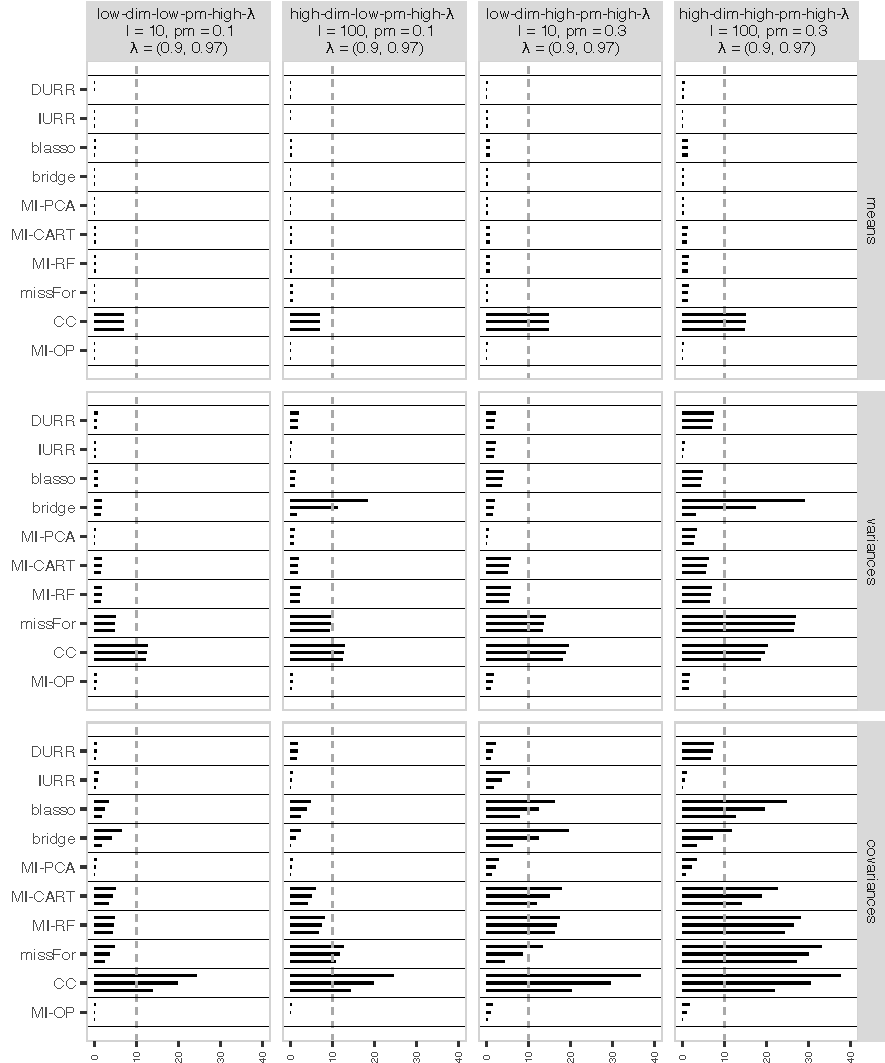
\includegraphics{../../output/graphs/exp2_semR_bias_14_summy.pdf}
\caption{PRBs for the means, variances and covariances (PRB) for condition 1 to 4.
	Conditions 1 to 4 correspond to the labels low-dim-low-pm-high-$\lambda$, high-dim-low-pm-high-$\lambda$, 
	low-dim-high-pm-high-$\lambda$, and high-dim-low-high-low-$\lambda$ in Table \ref{tab:condExp2}.
}
\label{fig:exp2bias14}
\end{figure}

\begin{figure}
	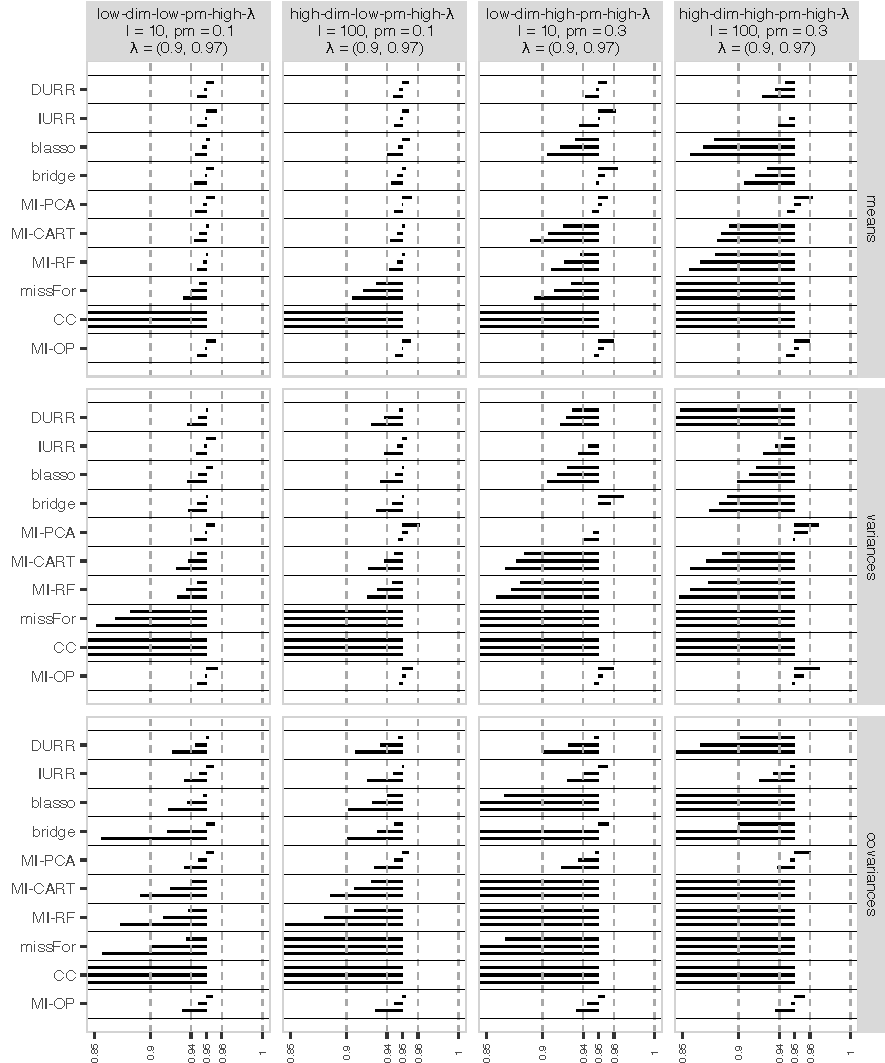
\includegraphics{../../output/graphs/exp2_semR_ci_14_summy.pdf}
\caption{CIC for the means, variances, and covariances for condition 1 to 4.
	Conditions 1 to 4 correspond to the labels low-dim-low-pm-high-$\lambda$, high-dim-low-pm-high-$\lambda$, 
	low-dim-high-pm-high-$\lambda$, and high-dim-low-high-low-$\lambda$ in Table \ref{tab:condExp2}.
}
\label{fig:exp2cir14}
\end{figure}

\begin{figure}
	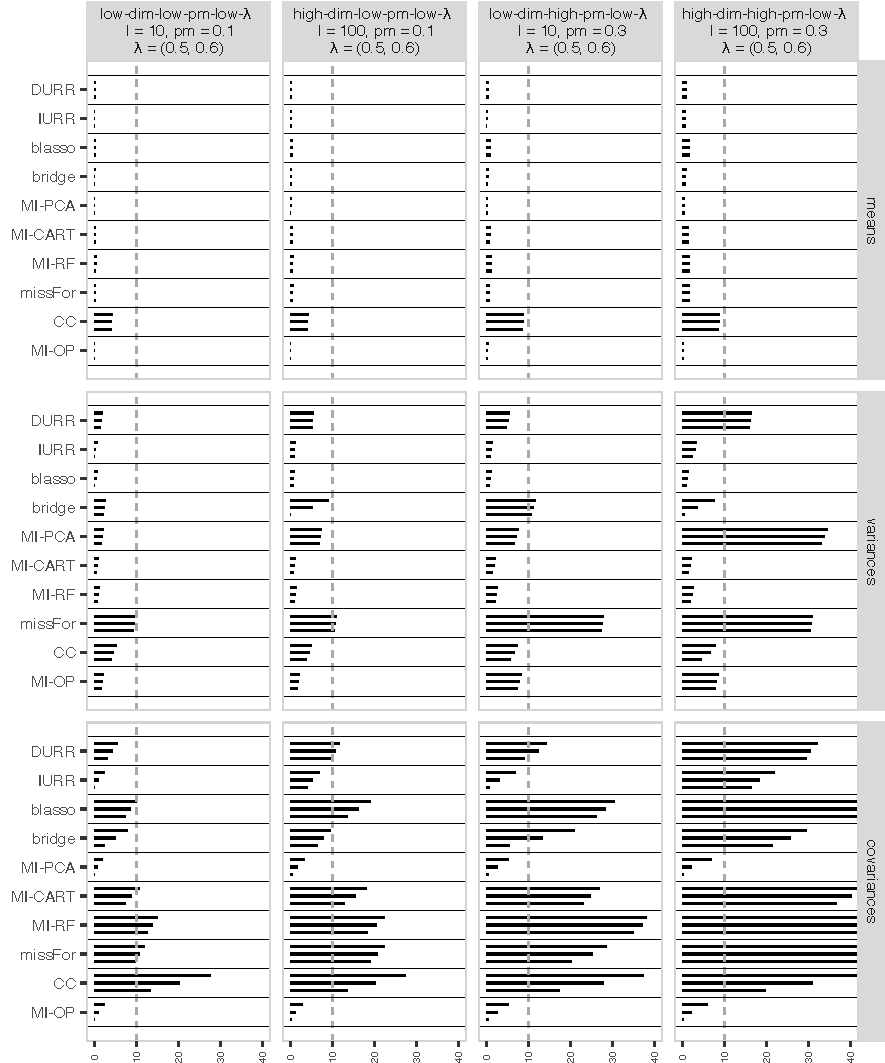
\includegraphics{../../output/graphs/exp2_semR_bias_58_summy.pdf}
\caption{PRBs for the means, variances and covariances (PRB) for condition 1 to 4.
	Conditions 5 to 8 correspond to the labels low-dim-low-pm-low-$\lambda$, high-dim-low-pm-low-$\lambda$, 
	low-dim-high-pm-low-$\lambda$, and high-dim-low-pm-low-$\lambda$ in Table \ref{tab:condExp2}.
}
\label{fig:exp2bias58}
\end{figure}

\begin{figure}
	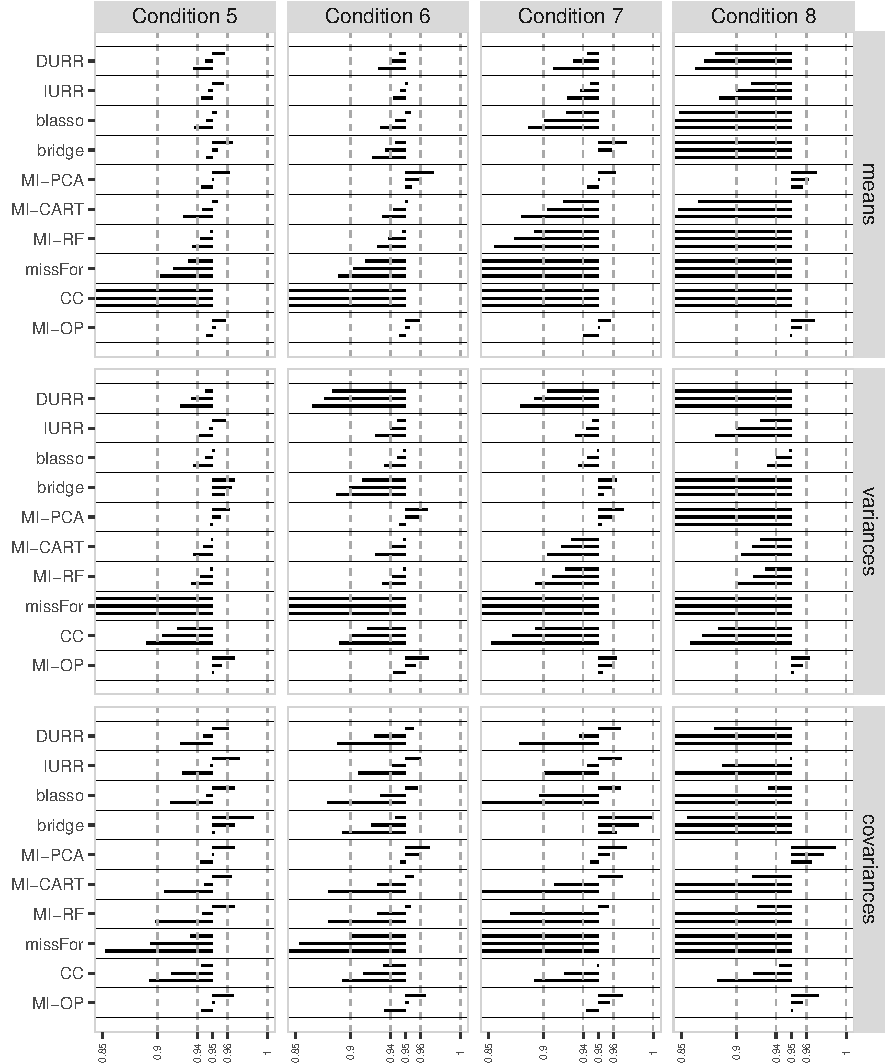
\includegraphics{../../output/graphs/exp2_semR_ci_58_summy.pdf}
\caption{CIC for the means, variances, and covariances for condition 1 to 4.
	Conditions 5 to 8 correspond to the labels low-dim-low-pm-low-$\lambda$, high-dim-low-pm-low-$\lambda$, 
	low-dim-high-pm-low-$\lambda$, and high-dim-low-pm-low-$\lambda$ in Table \ref{tab:condExp2}.
}
\label{fig:exp2cir58}
\end{figure}

\FloatBarrier

	\paragraph{Factor Loadings}
	Figure \ref{fig:exp2fl14} shows the average, minimum, and maximum PRB values for all the factor loadings 
	estimated by the Confirmatory Factor Analysis described above. 
	Most MI-Methods provided acceptably low bias for these estimates in all conditions except the high-dim-high-pm 
	ones (column 4).
	MI-OP, IURR, and MI-PCA outperformed all other methods and produced virtually unbiased estimates
	of the factor loadings in all conditions.
	Furthermore, MI-PCA outperformed IURR when factor loadings were low (panel b), maintaining inconsequential 
	biases even when data were high-dimensional and the proportion of missing values was high.

\begin{figure}
	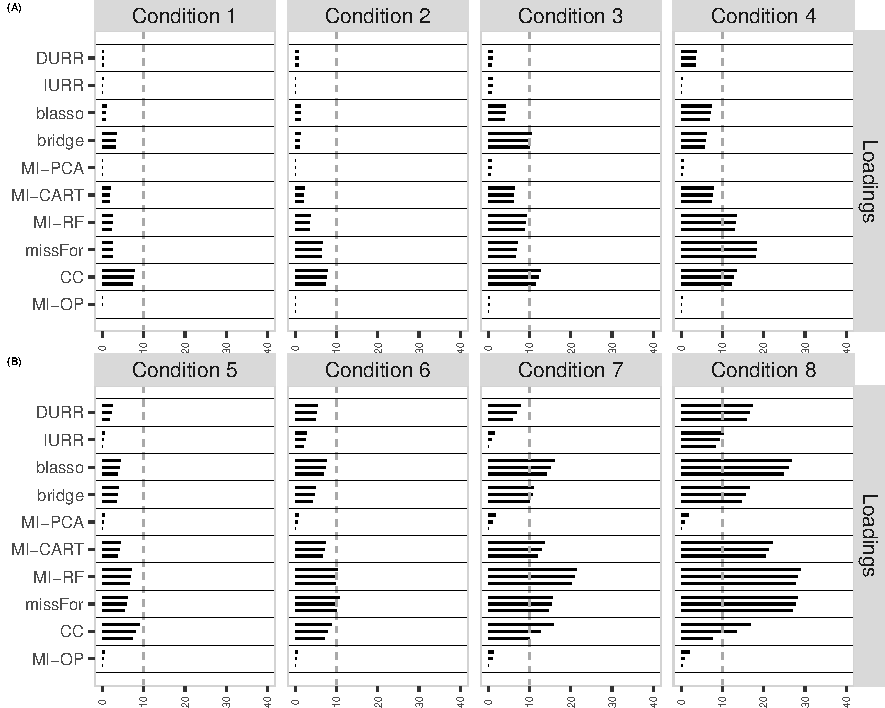
\includegraphics{../../output/graphs/exp2_CFA_lambda_BPR_summy.pdf}
	\caption{
		Percent Relative Bias (PRB) for the factor loadings in conditions 1 to 4 (panel A) 
		and conditions 5 to 8 (panel B).
		Conditions 1 to 8 correspond to the labels in Table \ref{tab:condExp2}.
		}
\label{fig:exp2fl14}
\end{figure}

\FloatBarrier % stops fig:exp2fl to leave its section

